% \documentclass[conference,10pt]{ieeeconf}
\documentclass[letterpaper, 10 pt, conference]{ieeeconf}
\IEEEoverridecommandlockouts
\overrideIEEEmargins
\usepackage{pstricks}
\usepackage{ifplatform}
\usepackage{xkeyval}
\usepackage{rotating}
\newtheorem{remark}{Remark}
\usepackage{graphics} % for pdf, bitmapped graphics files
% TEST-DEL: \usepackage[off]{auto-pst-pdf}
% \usepackage{mathptmx} % assumes new font selection scheme installed
\usepackage{times} % assumes new font selection scheme installed
\usepackage{amsmath} % assumes amsmath package installed
\usepackage{psfrag}
\usepackage{cancel}
\def\etal{\mbox{et al.}}
% \usepackage{pifont}
% \usepackage{flushend}
\usepackage[normalem]{ulem}
\usepackage{cite}
\usepackage{url}
\usepackage{color}
\input rgb
\def\blue#1{\textcolor{blue}{#1}}
\def\red#1{\textcolor{red}{#1}}
\def\orange#1{\textcolor{orange}{#1}}
\def\green#1{\textcolor{darkgreen}{#1}}
\usepackage{comment}
\usepackage{amssymb}
\usepackage{amsfonts}
%\usepackage[caption=false,font=footnotesize]{subfig}
\usepackage{subcaption}
% \usepackage{mathptmx}
%\usepackage{enumitem}
\usepackage{algorithmic}
\usepackage{algorithm}
\usepackage{pifont}% http://ctan.org/pkg/pifont
\newcommand{\cmark}{\ding{51}}%
\newcommand{\xmark}{\ding{55}}%
\newcommand{\smark}{$\bigstar$}%
\usepackage{booktabs}
%\input lamacro
\usepackage{lipsum}
\usepackage{array}
\newcolumntype{P}[1]{>{\centering\arraybackslash}p{#1}}
\newcommand{\JT}[1]{\textcolor{blue}{JT: #1}}
\newcommand{\AC}[1]{\textcolor{green}{AC: #1}}
\newcommand{\LP}[1]{\textcolor{red}{}}
\newcommand{\MN}[1]{\textcolor{orange}{MN: #1}}

\newcommand{\GR}[1]{\textcolor{magenta}{GR: #1}}
\newcommand{\assigned}[1]{\textcolor{purple}{Assigned To: #1}}
\newcommand{\budget}[1]{\textcolor{purple}{Page Budget: #1}}

\newcommand{\longonly}[1]{}
\newcommand{\shortonly}[1]{#1}

\newcommand{\maybeRemove}[1]{{\color{gray}#1}}
\newcommand{\xxx}{\textbf{\color{red}???}}
\newcommand{\LPafter}[1]{\longonly{\LP{#1}}}

% \renewcommand{\LP}[1]{}



\let\clipbox\relax
\usepackage{adjustbox}
%\usepackage{array}
\usepackage{booktabs}

\usepackage{CJKutf8}

\newcolumntype{R}[2]{%
    >{\adjustbox{angle=#1,lap=\width-(#2)}\bgroup}%
    l%
    <{\egroup}%
}
\newcommand*\rot{\multicolumn{1}{R{70}{1em}}}

\graphicspath{{figures/},{figures/new_diagrams/}}
\newcommand{\svgpath}{./images}

\usepackage{hyperref}
%\let\oldsection\section
%\renewcommand{\section}{\clearpage\oldsection}

%\allowdisplaybreaks[2]
\renewcommand{\baselinestretch}{0.97}
\textfloatsep = 6pt

% \let\subparagraph\relax
% \usepackage{titlesec}
% \usepackage[compact]{titlesec}
% \titlespacing{\section}{0pt}{2ex}{1ex}
% \titlespacing{\subsection}{0pt}{1ex}{0ex}
% \titlespacing{\subsubsection}{0pt}{0.5ex}{0ex}

\usepackage{mdwlist}
\let\stditemize\itemize
\let\endstditemize\enditemize
\let\itemize\undefined
\makecompactlist{itemize}{stditemize}

\let\stdenumerate\enumerate
\let\endstdenumerate\endenumerate
\let\enumerate\undefined
\makecompactlist{enumerate}{stdenumerate}

\setlength{\abovecaptionskip}{1pt}
\setlength{\belowcaptionskip}{1pt}

\usepackage[tracking=false,kerning=true,spacing=true]{microtype}
\pdfprotrudechars=2
\pdfadjustspacing=2

\title{\LARGE \bf
核災應變機器人 \\
Nuclear Disaster Strain Robot}

\author{李聖誠、張博凱\\
Sheng-Cheng Lee, Po-Kai Chang}
% <-this
% % stops a space
%\thanks{*This work was supported by Ministry of Science and Technology (MOST),
% Taiwan}% <-this % stops a space


\begin{document}
%\begin{CJK}{UTF8}{bsmi}
\begin{CJK}{UTF8}{bkai}

\maketitle

\thispagestyle{empty}
\pagestyle{empty}

%%%%%%%%%%%%%%%%%%%%%%%%%%%%%%%%%%%%%%%%%%%%%%%%%%%%%%%%%%%%%%%%%%%%%%%%%%%%%%%%

\begin{abstract}

無人載具為各國之國防科技發展重點,本計畫重點在無人載具之軟硬體系統開發整合,在過去研究中,將演算法部署到各種實體無人載具為重要工作,但往往因系統版本、硬體規格等執行不易,特別是在各種戶外場域。本研究使用機器人作業系統(Robot Operating System, ROS),為近年推展之ROS-Military基礎,鑑於近年美國國防高等研究計劃署 (Defense Advanced Research Projects Agency, DARPA)使用Gazebo進行機器人競賽,本計畫首先建立機器人模型於Gazebo虛擬平台,進而設計立體視覺感測器,分析點雲及開發演算法於地形模擬建構,以開發適合崎嶇地形之運動規劃。最後,在微小化實體平台進行測試,未來將進一步部署於大型無人載具進行實際場域驗證,如戶外斜坡/草地/道路之沿路自主導航測試,本計畫也將所設計的演算法與感測裝置放置於水面無人載具,進行機器人避障自主導航測試,並將參與2018年在夏威夷舉行 的RobotX機器人競賽。 

關鍵詞:無人載具、自主導航、RobotX競賽。

Autonomous robotic software and hardware systems have been developed in military research in the field for decades. Recently the rise of robot operating system (ROS) facilitates the development (ROS-Military) across academia, industry, and government organizations. Nevertheless, the challenges making software packages of autonomous navigation available to unmanned vehicles remain, especially in the outdoor fields. This work aims to develop essential functionalities of autonomous navigation, from simulation (Gazebo) to real-world rough terrains and water/ocean environments. We develop a method for mapping uneven surfaces and obstacles with triangular meshes, given the fusion of point clouds over time. We compared several motion planning approaches in efficiency and desired tasks. We have deployed the software on a miniaturized mobile platform in a controlled environment, and will further test the system using full-sized unmanned ground and surface vehicles. Some of the work will be used for the Team NCTU participations of the RobotX competition in Hawaii in 2018.

Keywords: Unmanned System, Autonomous Navigation, RobotX Challenge

\end{abstract}


%%%%%%%%%%%%%%%%%%%%%%%%%%%%%%%%%%%%%%%%%%%%%%%%%%%%%%%%%%%%%%%%%%%%%%%%%%%%%%%%
\section{前言}

隨著智慧型機器人與人工智慧的蓬勃發展,近年來各國均投入於無人載具之開發與研究,已經在非常多場域漸漸出現。在有結構性的環境(structured environments)下,無人駕駛車在從室外之高速公路、郊外人車較少之公路,到室內工廠物流運輸機器人系統已經有相當成熟的發展,其原因在於其所產生的應用是非常貼切人類的日常生活,並且能創造更大之經濟效應,例如:交通工具、商業物流等。但在意外發時,例如:輻射外洩。等人類無法進入之嚴峻場地,機器人更能發揮其不可取代性,代替人類進入災區進行移動、導航、定位、救援。

\begin{figure}[t]
  \centering
    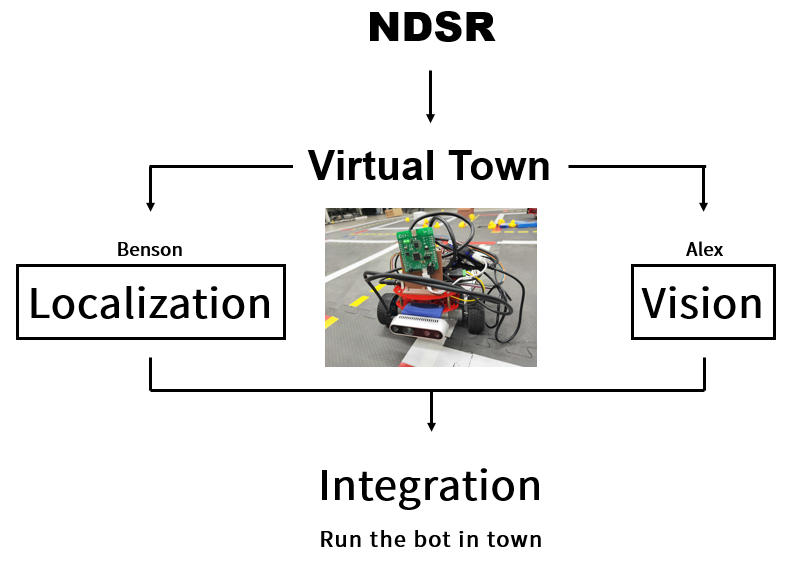
\includegraphics[width=\columnwidth]{images/teaser.png}
        \caption{本計畫目標為建置整合機器人搜救系統,包括UWB定位及MobileNet-SSD目標偵測,能夠清楚知道目標搜救物位於地圖中的何處,於Duckietown場地進行驗證。}
 \label{figure:teaser}
\end{figure}

國防科技一直以來是各個國家的發展重點。美國國防高等研究計劃署 (Defense Advanced Research Projects Agency, DARPA)以及美國太空總署(NASA)針對這樣的挑戰, 舉辦相關競賽,如:DARPA Subterranean Challenge(簡稱SubT),這場競賽旨在開發能夠「探索快速繪製、導航、搜索和開發複雜地下環境的新方法」,包括人造隧道系統、城市地下和自然洞穴網絡等。大賽要求參賽者研製出能幫助人類在地下導航、繪圖以及搜尋的系統,所有救援系統在地下結構發生塌方或其他災難時,能夠在對人類來說有危險的地方移動和導航,幫助救援。

而本次專題就是根據核災發生現場,或任何人員無法進入之場地、城市,由應變機器人進入災區偵測目標物,並且能夠在無GPS之場域進行定位,準確得知無人車輛目前位置與目標物之相對位置,讓搜救人員迅速進行偵查、救援。

\begin{figure*}[tb]
	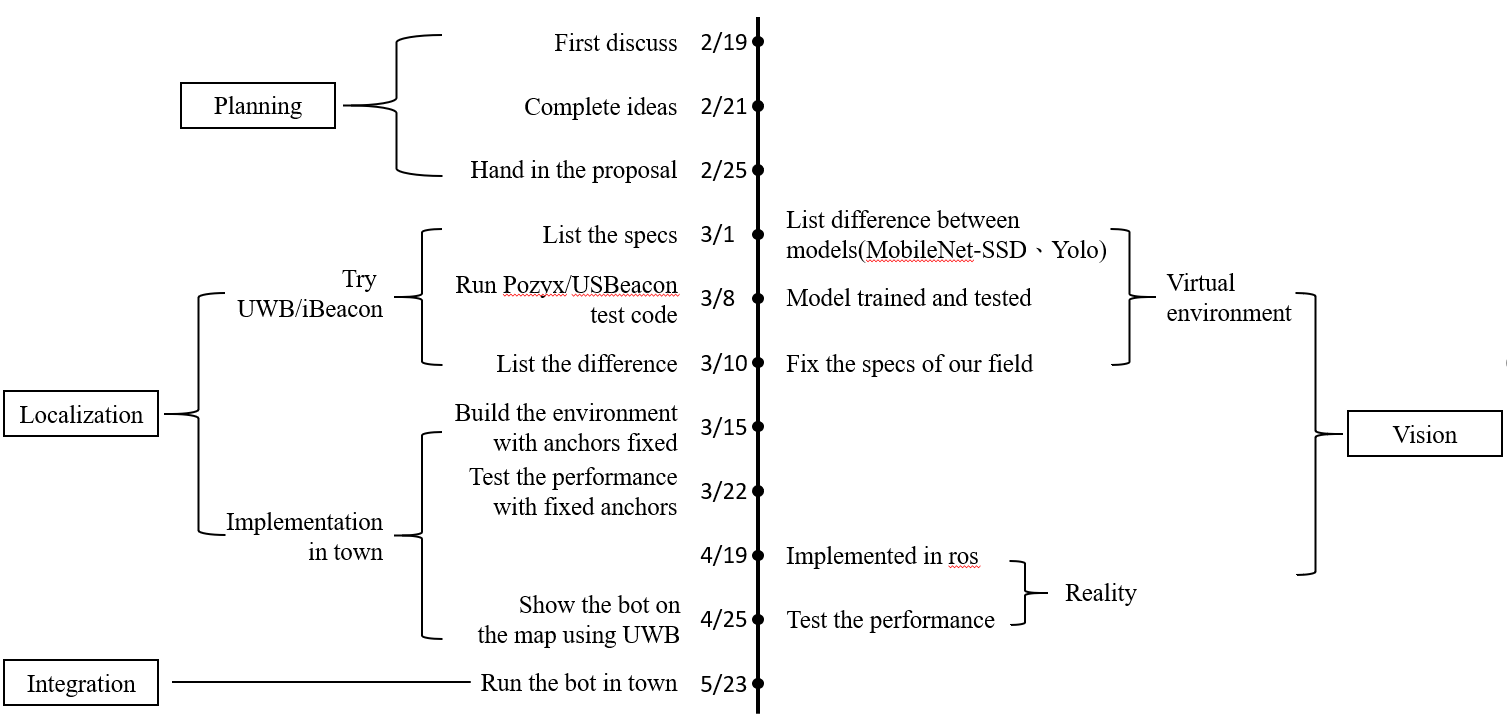
\includegraphics[width=1.8\columnwidth]{images/sys-architecture.png}
	\centering
	\caption{本專題之進度分工圖,博凱-Vision、聖誠-Localization}
	\label{figure:localization_sys_architecture}
\end{figure*}

綜合上述,此搜救機器人需具備立體視覺整合系統感知偵測目標物並與UWB定位結合,需考量目標物大小、定位準度、目標物深度資訊等等計算出相對位置,因此,本報告的目標與貢獻如下:

\begin{enumerate}
\item
UWB定位及MobileNet-SSD目標辨識
\item 
合併且整合系統
\item 
將結果可視化並顯示於Rviz
\end{enumerate}









\section{核災應變機器人設計}
為了模擬發生核災的城市,我們利用MIT Duckietown的巧拼建置縮小版核災城市,以scale down之環境呈現核災發生後人類無法進入之城市。城市大小訂為5*5之巧拼,每片巧拼60cm,城市總大小300cm*300cm。
在這樣的城市中,我們的機器人要能夠辨識受害者及周遭環境,並且定位出自己所在的位置,才能夠發揮核災應變的功效。所以本次的專題,我們主要心力就放在視覺(Vision)以及定位(Localization)這兩項。

\begin{figure}[h]
  \centering
    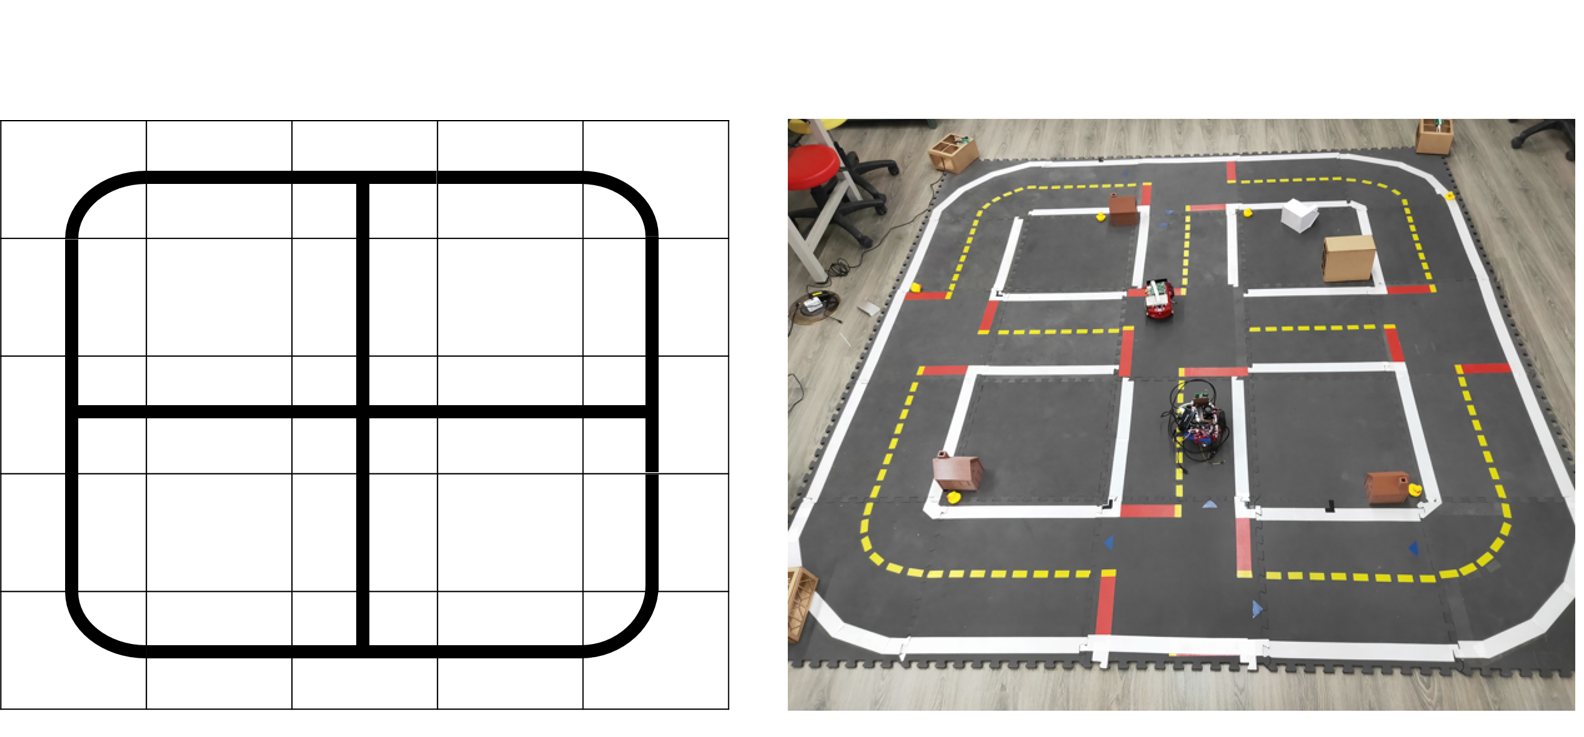
\includegraphics[width=\columnwidth]{images/field.png}
        \caption{模擬城市場地設計}
 \label{figure:field}
\end{figure}

\subsection{Localization}
我們採用Ultra-wideband作為取得定位資訊的裝置,使用pypozyx函式庫,利用UWB Anchor的訊號強度與TWR(Two Way Ranging)定位技術(圖\ref{figure:uwb_tech})~\cite{7491981}同時利用三個以上的Anchor裝置就能定位出2D座標,同時利用四個以上能定位3D座標。同時UWB裝置上也搭載IMU感測器,能夠知道UWB裝置的方向。結合位置與方向這兩樣資訊我們能夠得出固定在車上的TAG三維姿態(Pose)。

\begin{figure}[h]
  \centering
    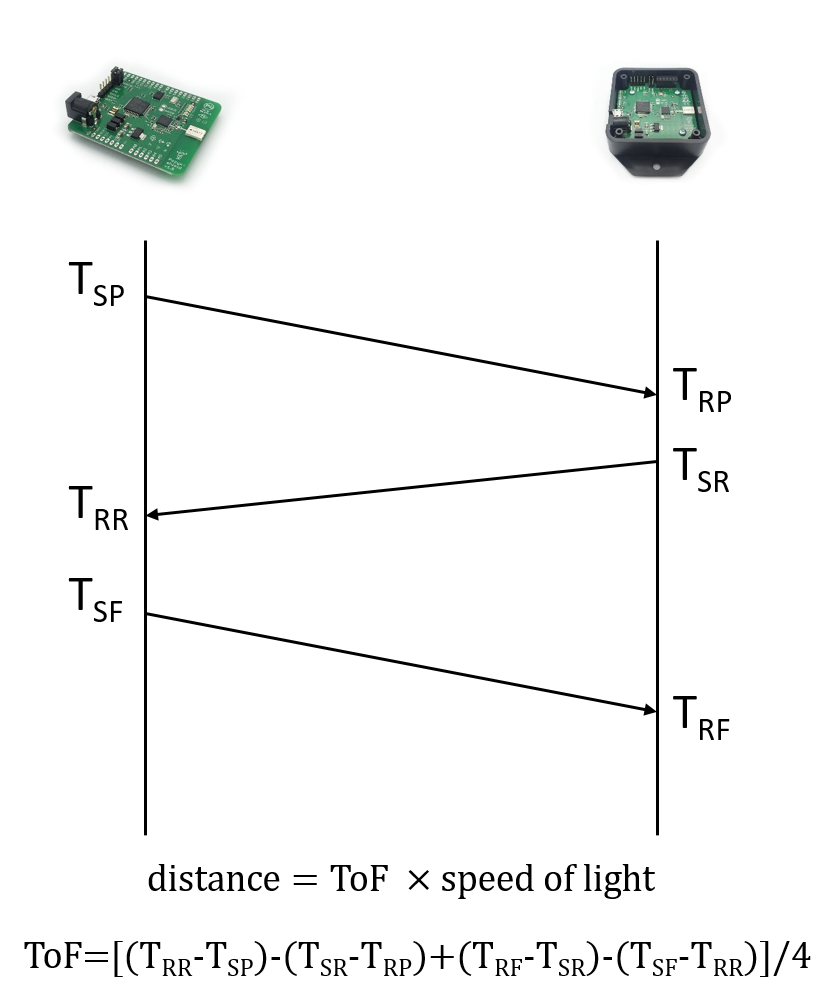
\includegraphics[width=\columnwidth]{images/uwb_tech.png}
        \caption{UWB Localization TWR technique}
 \label{figure:uwb_tech}
\end{figure}

\subsection{Vision}
在核災中,我們必須辨識出該城市內之物品,找出可能的目標物品以及生還者。
由於此次人本專題我們使用了Duckietown城市模擬核災發生並作為驗證場地,所以重新組裝了一台Super Duckiebot。
在視覺部份因考量到車體大小,故選擇使用體積較小的Jetson Nano處理相關視覺運算,同時也使用運算量較小的MobileNet-SSD Model,在影像辨識部份利用RGB資訊進行Training,精準度、輕巧度及靈敏度是Artifact search相當重要的指標,控制訓練後Model的大小將其放置於較輕巧的Jetson Nano上運行,並且考量到幀數(FPS)也就是一秒讀取幾張圖片進行辨識,各個環節環環相扣。

當辨識出目標物後,隨即使用Depth資訊利用投影矩陣取得目標物與相機之相對座標,結合UWB定位所取得之姿態訊息,定位出目標物之絕對位置,最後呈現於Rviz。

\begin{figure}[h]
  \centering
    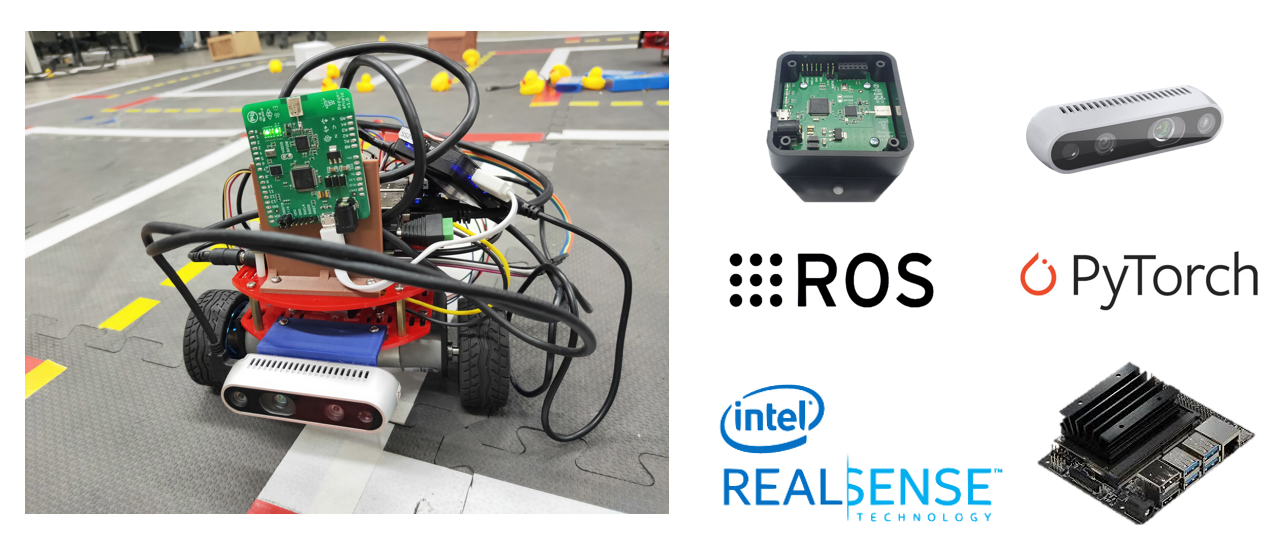
\includegraphics[width=\columnwidth]{images/car.png}
        \caption{車體設計及相關環境}
 \label{figure:car}
\end{figure}











\section{系統設計}

\subsection{機器人硬體設計}
機器人的車體部分,我們沿用MIT Duckietown之車架壓克力板,但是為了更好的載重量我們將馬達改成具有編碼器之馬達,除了增加穩定性與馬力以外,未來也可加入Wheel Odometry之功能提供更完整的SLAM。主控板部分我們使用Nvidia發行之Jetson Nano,具有強大的圖形運算能力,能為深度學習的Model提供更可靠的運算處理。為了能夠定位以及辨識物體,我們在車上加上Pozyx公司推出的UWB裝置,以及Intel RealSense的D435深度相機。前者能夠提供3D Pose定位後者能夠提供RGBD之深度影像有利於視覺辨識與計算物體相對位置。


\begin{figure}[h] % h means put this image here
  \centering
    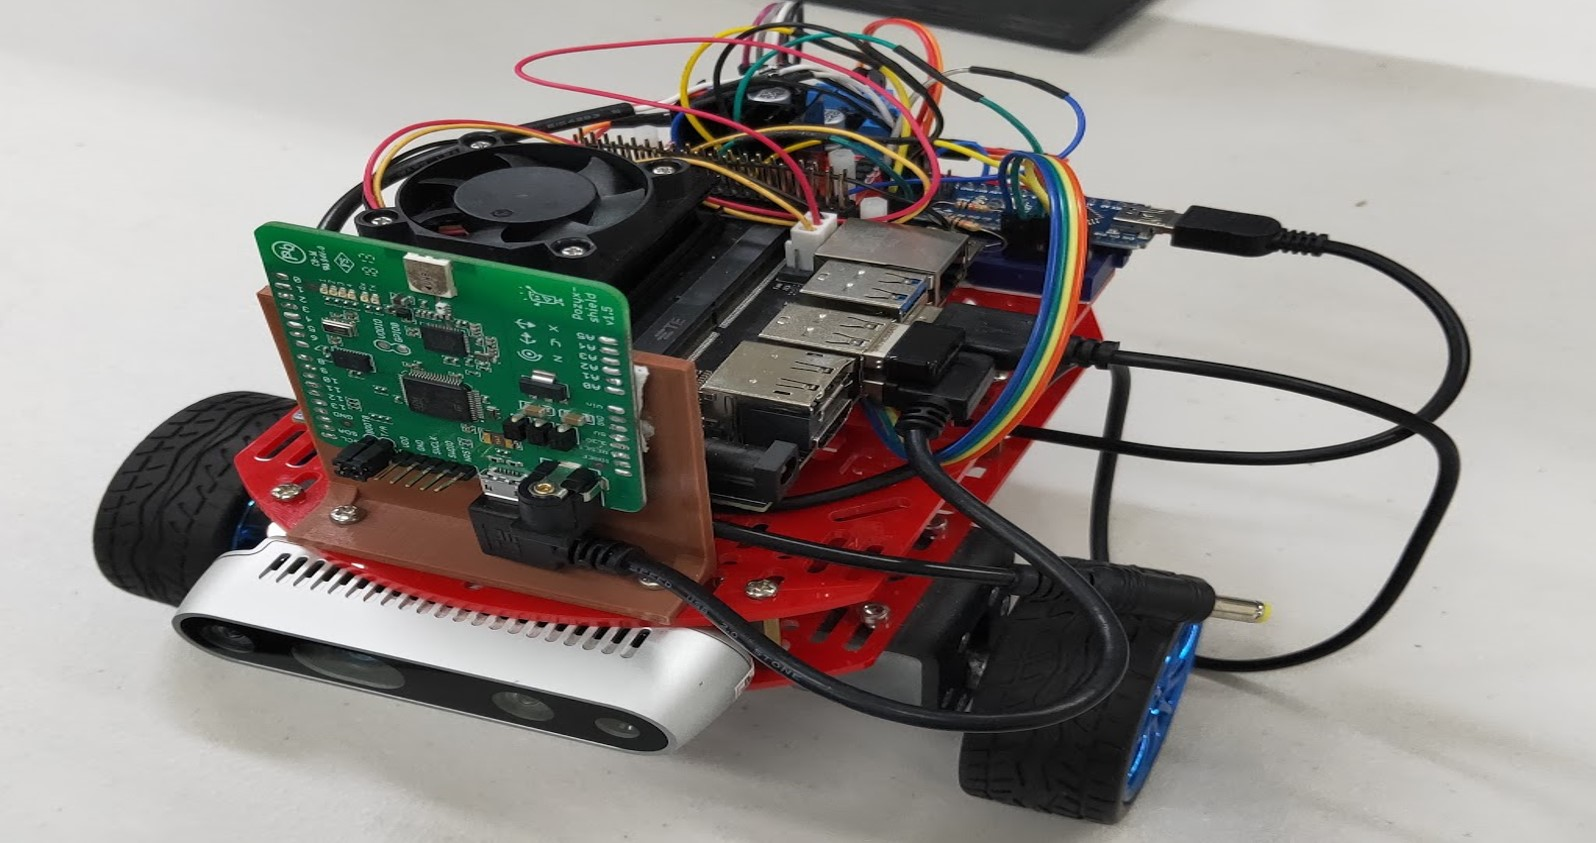
\includegraphics[width=0.8\columnwidth]{images/jetson-car_2.jpg}	
      \caption{核災應變機器人之硬體設計}
    \label{figure:car2}
\end{figure}

\subsection{機器人作業系統}
在機器人上運行的系統,我們安裝Ubuntu18.04與ROS Melodic。ROS(Robot Operating System)是專為機器人軟體開發所設計出來的一套電腦作業系統架構。它是一個開源的元級作業系統,提供類似於作業系統的服務,包括硬體抽象描述、底層驅動程序管理、共用功能的執行、程序間消息傳遞、程序發行包管理,它也提供一些工具和庫用於獲取、建立、編寫和執行多機融合的程序。
利用ROS我們能夠快速建立各種Node並利用Publisher與Subscriber互相傳送資訊。

\subsection{機器人定位與移動}
我們用pypozyx的函式庫取得Tag Pose並且Publish至ROS topic,另一個Node將每個Pose記錄下來後,可在地圖上畫出一個行進軌跡,方便搜尋到物品之後進行後續的動作。
機器人的移動是利用ROS的Joy Package搭配ROS Serial將car command傳送至Arduino驅動馬達,達到利用Joystick控制車子行進之功能。

\subsection{機器人視覺與物品定位}
抽取D435之RGB影像後,首先使用MobileNet-SSD進行物品辨識,我們將搜索到的物品在畫面中標出Bounding Box之後,利用Depth資料以及CameraInfo將影像投影至三維空間,標出物品相對位置以後,利用TF函式乘上Pozyx的Pose資訊,

\begin{figure}[h] % h means put this image here
  \centering
    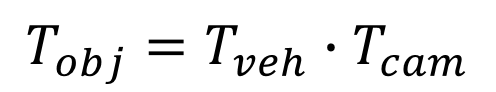
\includegraphics[width=0.8\columnwidth]{images/tf.png}	
      \caption{物品座標轉換}
    \label{figure:tf}
\end{figure}

\section{實驗與實體驗證}

\subsection{機器人定位}

此專題以室內高精準度定位為目標,配合深度相機之影像辨識與物體深度,找到目標物之位置並標記。

\paragraph{定位準確度測試}

本專題之定位裝置使用Ultra-wideband超寬頻通訊天線,為提供目標物位置之量測精準度,設計此定位精準度測試。鋪設5*5巧拼,量測各點之UWB定位座標,比較Ground Truth,進行多次量測後計算方均根值作為誤差數據,實驗結果如表
\ref{table:localization_error}所示。將結果之數據量化後標示於地圖上如圖\ref{figure:localization_result}所示。

\begin{table}[h]
	\centering
	\begin{tabular}{| c| c| c|}
		\hline
		Ground Truth X (m) & Ground Truth Y (mm) & 定位誤差 (mm) \\ 
		\hline
		300 & 300 & 68.43 \\ 
		\hline
		1500  & 300 & 117.58 \\ 
		\hline 
		2700  & 300 & 64.69 \\ 
		\hline 
		2700  & 1500 & 195.94 \\ 
		\hline 
		2700  & 2700 & 220.11 \\ 
		\hline 
		1500  & 2700 & 200.33 \\ 
		\hline 
		300  & 2700 & 56.93 \\ 
		\hline 
		300  & 1500 & 27.56 \\ 
		\hline 
		1500  & 1500 & 50.39 \\ 
		\hline 
	\end{tabular}
	\caption{定位測試}
	\label{table:localization_error}
\end{table} 

\begin{figure}[bht]
	\centering
	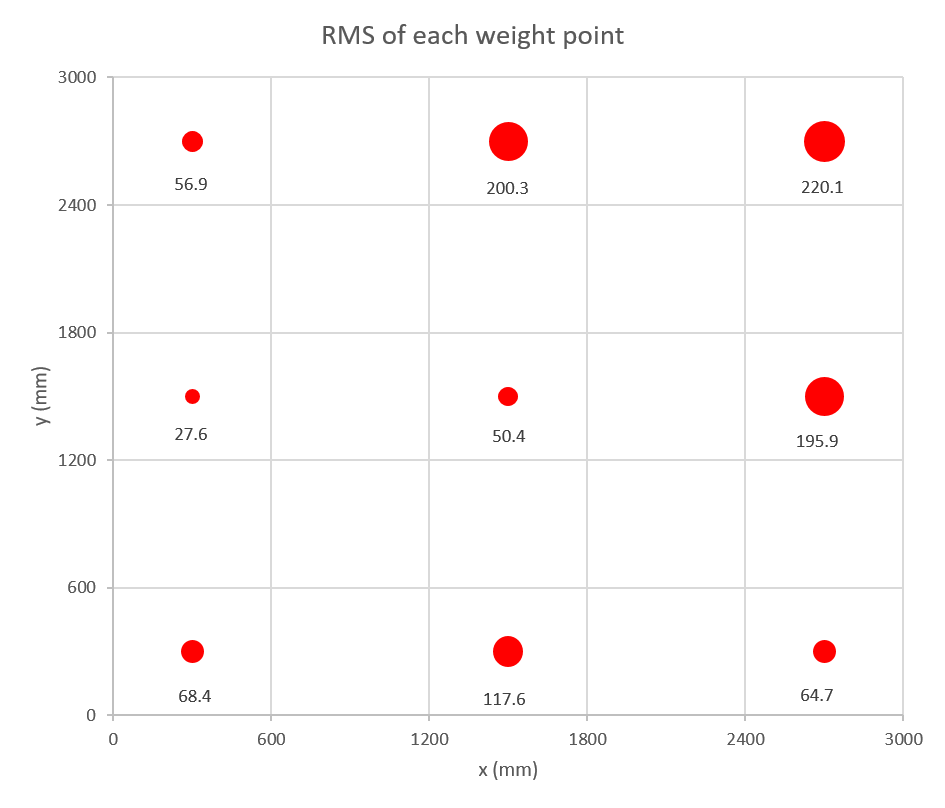
\includegraphics[height=!,width=\linewidth,keepaspectratio=true]
	{images/uwb_bench.png}
	\caption{以UWB定位之誤差量測實驗結果}
	\label{figure:localization_result}
\end{figure}

\paragraph{定位測試影片} 

本專題利用UWB之定位結果經過移動限制過濾器後繪製出行進軌跡,測試影片連結如下:

\begin{itemize}

\item
載具利用遙控行進場地一圈並繪製出軌跡圖
\url{<Put URL Here>}

\item
避障實驗一(靜態障礙物): 
\url{https://youtu.be/ve4Mln4D1xo}

\end{itemize}


\subsection{影像辨識}

本專題比較目標物於各版本SSD運算量及FPS後,如\ref{table:fps_compare},選擇FPS較高且運算量較低的MobileNet-V1 SSD,使用Jetson Nano執行Model。
並配合深度相機於標記目標物後,將bounding box之中點位置利用矩陣投影的方式找出目標物與相機之距離,如\ref{figure:vision}。

由如\ref{figure:evaluation}可以發現到Duck的Average Precision會比其他的還要來的低只有0.58,明顯的看出MobileNet-SSD對於小物品的偵測相對於其他model如yolo較不理想。


\begin{table}[h]
	\centering
	\begin{tabular}{| c| c| c|}
		\hline
		Frame Rate (FPS) & desktop 1080 & Jetson Nano \\ 
		\hline
		SSD & 36 & 1.5 \\ 
		\hline
		MobileNet-V1 SSD  & 90-100 & 16.5 \\ 
		\hline 
		MobileNet-V2 SSD & 78-80 & 12 \\ 
 
		\hline 
	\end{tabular}
	\caption{各版本FPS比較}
	\label{table:fps_compare}
\end{table} 

\begin{figure}[t]
	\centering
	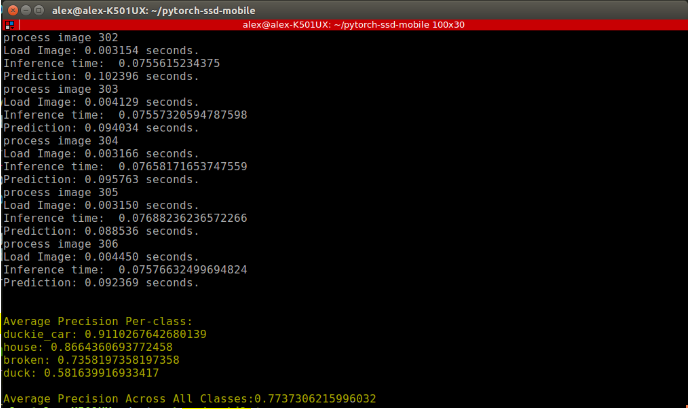
\includegraphics[height=!,width=\linewidth,keepaspectratio=true]
	{images/evaluation.png}
	\caption{MobileNet-V1 SSD evaluation}
	\label{figure:evaluation}
\end{figure}

\begin{figure}[h]
	\centering
	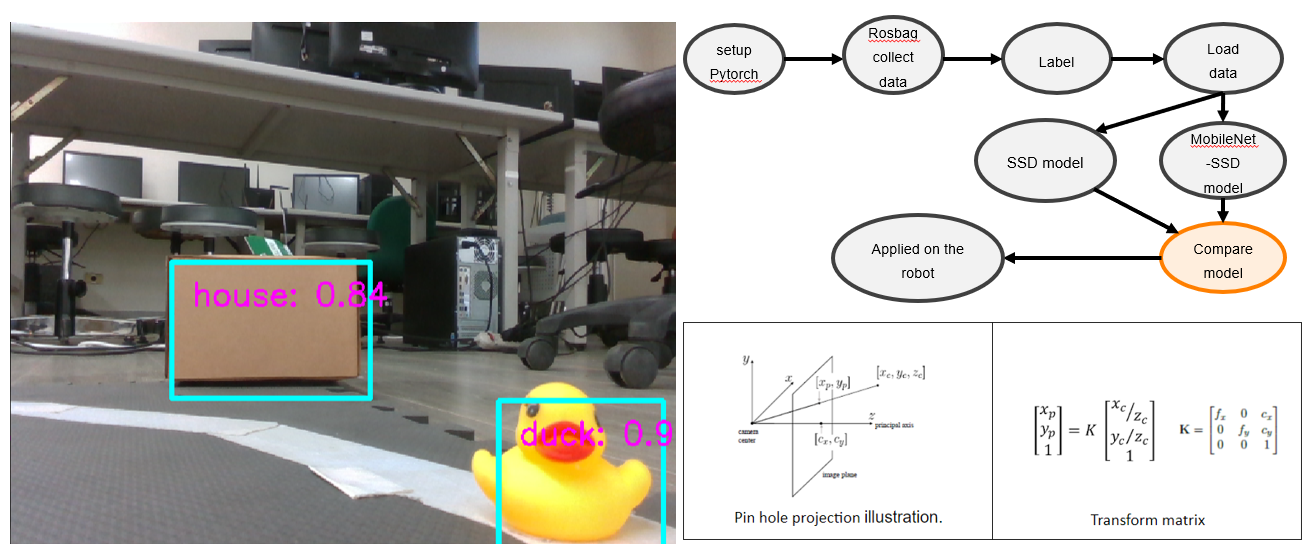
\includegraphics[height=!,width=\linewidth,keepaspectratio=true]
	{images/vision.png}
	\caption{預測目標物之實驗步驟及相對距離投影矩陣}
	\label{figure:vision}
\end{figure}




\section{結論}

本次專題,使用Duckietown之虛擬城市環境,設計小型探測車裝置,並開發影像辨識與定位之功能,從而瞭解系統運作原理以及學習使用定位與影像辨識之技術。本學期已達成物件辨識與定位之功能,未來希望能加入Lidar與編碼器馬達之SLAM技術,進行更準確之定位與搜救平台研究開發。

\begin{figure}[t]
	\centering
	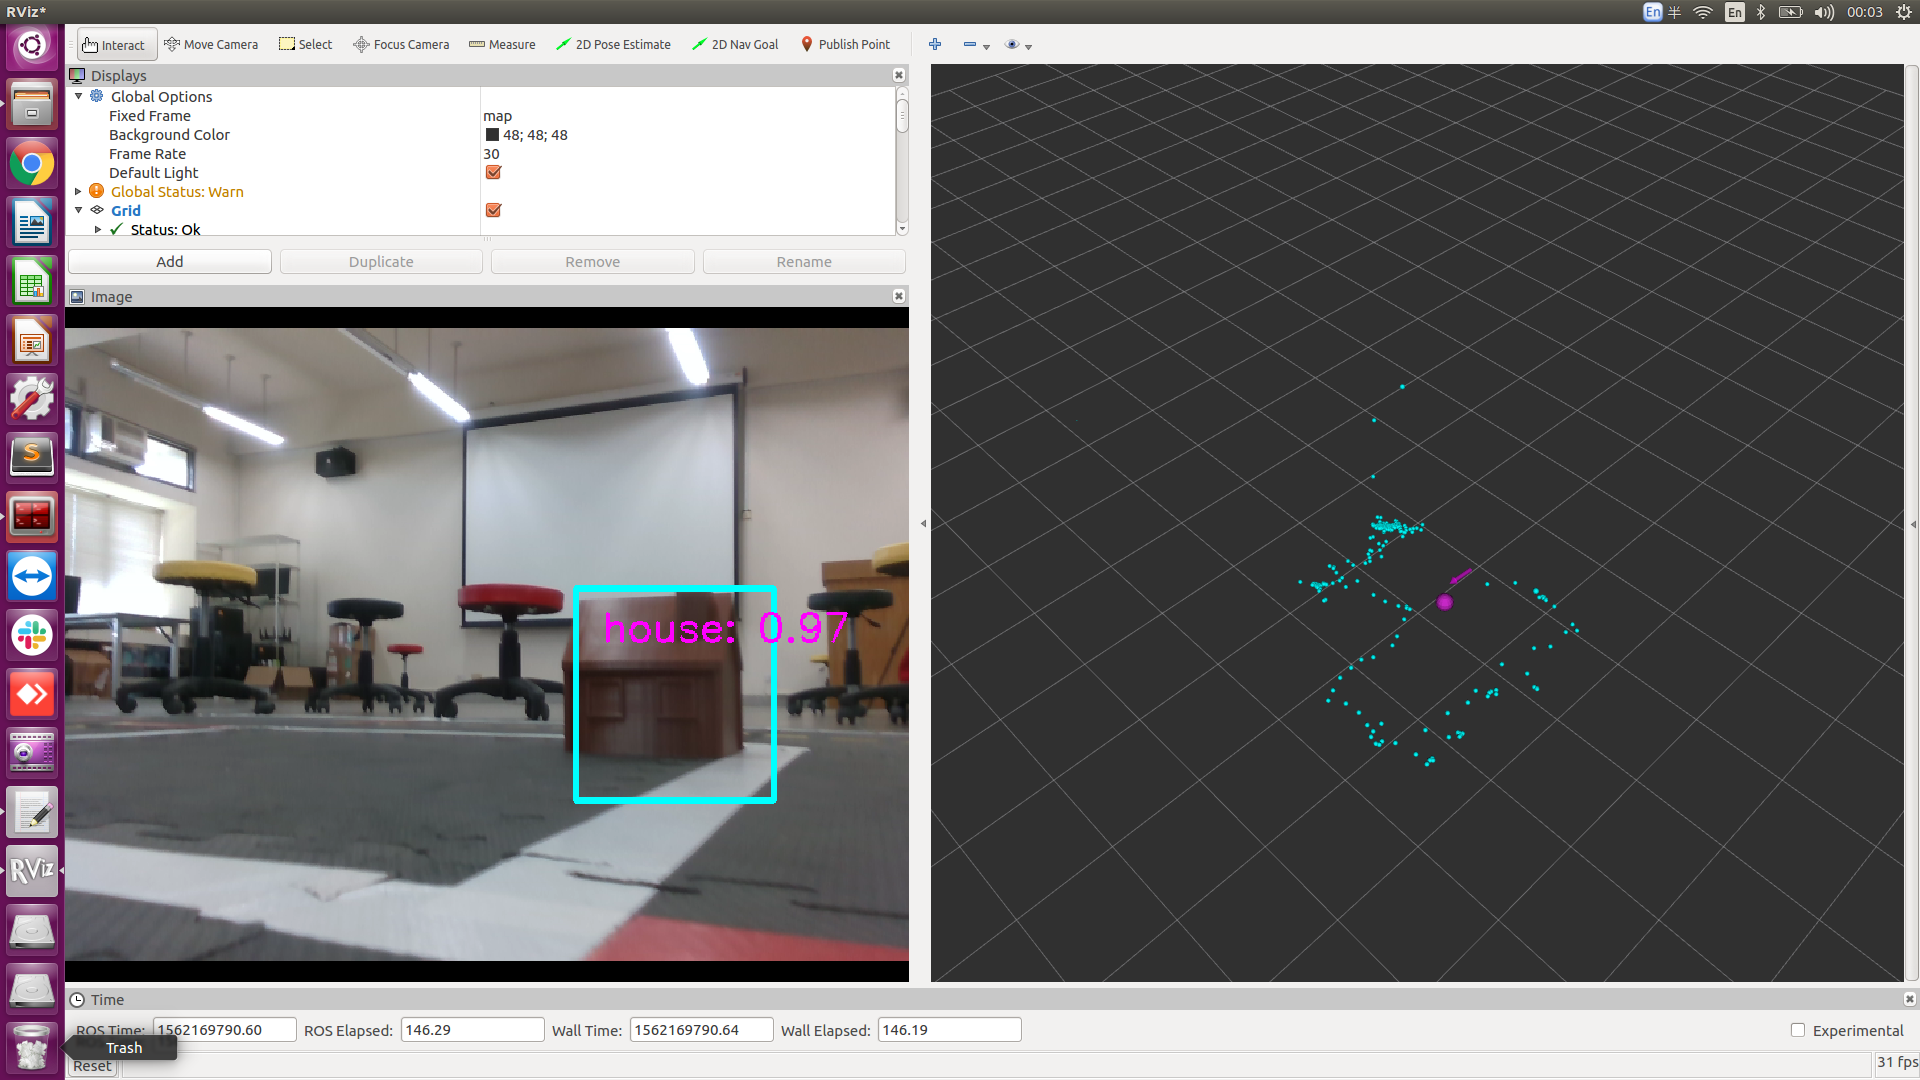
\includegraphics[width=\linewidth,keepaspectratio=true]
	{images/demo.png}
	\caption{專題成果呈現}
	\label{figure:demo_result}
\end{figure}


%\addtolength{\textheight}{-12cm} % This command serves to balance the column lengths
                                  % on the last page of the document manually. It shortens
                                  % the textheight of the last page by a suitable amount.
                                  % This command does not take effect until the next page
                                  % so it should come on the page before the last. Make
                                  % sure that you do not shorten the textheight too much.

%%%%%%%%%%%%%%%%%%%%%%%%%%%%%%%%%%%%%%%%%%%%%%%%%%%%%%%%%%%%%%%%%%%%%%%%%%%%%%%%
%\section*{APPENDIX}

%Appendixes should appear before the acknowledgment.


%This work was partially
%supported by the National Science Foundation under grants IIS-1318392 and
%IIS-1405259.

%%%%%%%%%%%%%%%%%%%%%%%%%%%%%%%%%%%%%%%%%%%%%%%%%%%%%%%%%%%%%%%%%%%%%%%%%%%%%%%%

\bibliographystyle{IEEEtran}
\bibliography{arg-egbib}

\end{CJK}
\end{document}
